\section{Image Synthesis Examples with CEP}
\label{sec:image_exp}

\begin{figure}[t]
\vspace{-.05in}
	\begin{minipage}{0.18\linewidth}
		\centering
			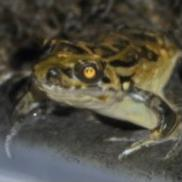
\includegraphics[width=\linewidth]{pics/color_imgs/main_color2_s0.0.jpg}\\
			\small{$s=0.0$} \\
	\end{minipage}
	\begin{minipage}{0.18\linewidth}
		\centering
			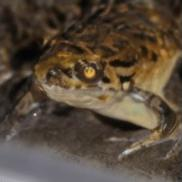
\includegraphics[width=\linewidth]{pics/color_imgs/main_color0_s1.0.jpg}\\
			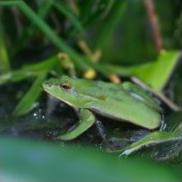
\includegraphics[width=\linewidth]{pics/color_imgs/main_color1_s1.0.jpg}\\
			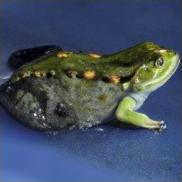
\includegraphics[width=\linewidth]{pics/color_imgs/main_color2_s1.0.jpg}\\
		  %
		    \small{$s=1.0$} \\
	\end{minipage}
	\begin{minipage}{0.18\linewidth}
		\centering
			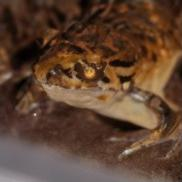
\includegraphics[width=\linewidth]{pics/color_imgs/main_color0_s2.0.jpg}\\
			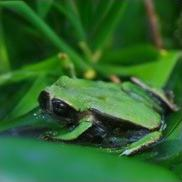
\includegraphics[width=\linewidth]{pics/color_imgs/main_color1_s2.0.jpg}\\
			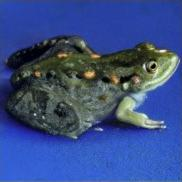
\includegraphics[width=\linewidth]{pics/color_imgs/main_color2_s2.0.jpg}\\
		  %
		    \small{$s=2.0$} \\
	\end{minipage}
	\begin{minipage}{0.18\linewidth}
		\centering
			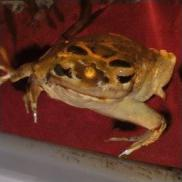
\includegraphics[width=\linewidth]{pics/color_imgs/main_color0_s3.0.jpg}\\
			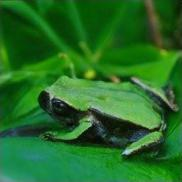
\includegraphics[width=\linewidth]{pics/color_imgs/main_color1_s3.0.jpg}\\
			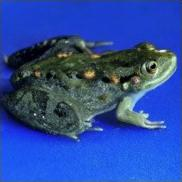
\includegraphics[width=\linewidth]{pics/color_imgs/main_color2_s3.0.jpg}\\
		  %
		    \small{$s=3.0$} \\
	\end{minipage}
	\begin{minipage}{0.18\linewidth}
		\centering
			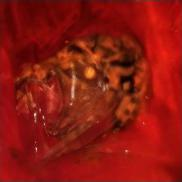
\includegraphics[width=\linewidth]{pics/color_imgs/main_color0_s10.0.jpg}\\
			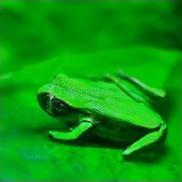
\includegraphics[width=\linewidth]{pics/color_imgs/main_color1_s10.0.jpg}\\
			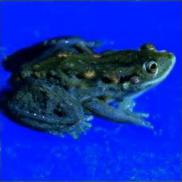
\includegraphics[width=\linewidth]{pics/color_imgs/main_color2_s10.0.jpg}\\
		  %
		    \small{$s=10.0$} \\
	\end{minipage}
	\begin{minipage}{0.04\linewidth}
		\centering
			\small{\rotatebox{90}{red}}\\
			\vspace{0.4in}
			\small{\rotatebox{90}{green}}\\
			\vspace{0.3in}
			\small{\rotatebox{90}{blue}}\\
	\end{minipage}
	\caption{\label{fig:main_color}\small{Samples by color guidance with red, green, and blue, varying the guidance scale $s$ (under a fixed random seed).}
}
\vspace{-.2in}
\end{figure}












\subsection{Results in Class-Conditional Image Synthesis}
\label{classifier_results}

We quantitatively evaluate our proposed method (\eqref{Eq:contarstive_condition_loss}) in image synthesis tasks on ImageNet as is shown in \cref{tab:guide2}. Our method achieves results that are roughly on par with classic classifier guidance \citep{diffusion_beat_gan}. We also qualitatively compare sampled images guided by our proposed CEP guidance and classifier guidance with fixed random seeds in \cref{fig:image_guidance_qualitative}, which shows that they generate samples that are almost visually identical. Besides the training objective, our method uses exactly the same network architecture, training pipeline, and evaluation methods as \citet{diffusion_beat_gan}, without any kind of hyperparameter tuning. These results empirically indicate that our method is an almost equally well-performing alternative to classifier guidance in ImageNet image synthesis tasks.

\subsection{Energy-Guided Image Synthesis}
This section showcases how image synthesis can be controlled through a continuous energy function as described in \eqref{Eq:target_distribution_intro} instead of a discrete class condition as in \cref{classifier_results}. We define the energy function at $t=0$ data space to indicate the overall color appearance of an image:
\begin{equation}
    \label{Eq:color_q0}
    \gE(\x) := - \overline{\| h(\x) - h_\textbf{tar} \|_1},
\end{equation}
where $h(\x)$ represents the hue value for each pixel in an image $\x$, and can be calculated via Hue-Saturation-Intensity (HSI) decomposition \citep{cvbook}.  $h(\x)$ is defined in an angular space of range $[0, 2\pi]$, where red is at angle $0$, green at $2\pi/3$, blue at $4\pi/3$, and red again at $2\pi$. As a result, by setting the target hue $h_\textbf{tar}$ to corresponding angular values, we can evaluate how an image is visually close to a ``pure color'' image.

With such a definition of the energy function, we train three energy guidance models to control the overall color appearance of sampled images. An illustration is given in \cref{fig:main_color}. By switching among different guidance models and tuning guidance scales to control the guidance effect similar to \citet{diffusion_beat_gan, ho2021classifier}, we can effectively control the color appearance of an image. If the diffusion prior is a conditional model, generated images might have different backgrounds (e.g., desert, forest, and sky) to meet different preferences of color appearance while ensuring fidelity. See more examples in \cref{Sec:Scale_samples}.
